% Foliensatz: "AFu-Kurs nach DJ4UF" von DK0TU, Amateurfunkgruppe der TU Berlin
% Lizenz: CC BY-NC-SA 3.0 de (http://creativecommons.org/licenses/by-nc-sa/3.0/de/)
% Autoren: Martin Deutschmann DM7MD <martin.deutschmann@campus.tu-berlin.de>, Lars Weiler DC4LW <dc4lw@darc.de>
% Korrekturen: Sebastian Lange <dl7bst@dk0tu.de>

\documentclass[aspectratio=169]{beamer}

\usepackage[ngerman]{babel} % deutsche Worttrennung etc.
\usepackage[utf8]{inputenc} % UTF8 Text

\usepackage[super, comma, numbers, square, sort]{natbib}

\usepackage{hyperref}       % Hyperref Package für bessere Referenzen (todo)
\hypersetup{
	colorlinks=false,       %   false: boxed links; true: colored links
    %linkcolor=white,       %   color of internal links (change box color with linkbordercolor)
    citecolor=red,          %   color of links to bibliography
    filecolor=white,        %   color of file links
    urlcolor=blue           %   color of external links
}

\usepackage{multirow}
\usepackage{wasysym}  % Math Symbols like \permil
%\usepackage{colortbl}
%\usepackage{subscript}
%\usepackage{caption}
%\usepackage{setspace}
%\usepackage{xcolor}        % benutze CodeListe

% Footnote
%\usepackage{hanging}
%
%\setbeamertemplate{footnote}{%
%  \hangpara{2em}{1}%
%  \makebox[2em][l]{\insertfootnotemark}\footnotesize\insertfootnotetext\par%
%}


%\usepackage{pgf}
%\usepackage{tikz}
%\usetikzlibrary{arrows,automata}
%\usetikzlibrary{positioning}
%
%\tikzset{
%    state/.style={
%           rectangle,
%           rounded corners,
%           draw=black, very thick,
%           minimum height=2em,
%           minimum width=2pt,
%           inner sep=2pt,
%           text centered,
%           },
%}

%\usepackage{listings}
%\lstset{basicstyle=\small, numberstyle=\tiny, extendedchars=true, numbers=left, numbersep=5pt}
%\lstset{showtabs=false, showspaces=false, showstringspaces=false}
%%\lstset{backgroundcolor=\color{white!75!lightgray}, , frame=single}
%%\lstset{backgroundcolor=\color{white}}
%%\lstset{backgroundcolor=none}
%\lstset{keywordstyle=\color{blue!50!gray},  identifierstyle=\color{black}}
%\lstset{commentstyle=\color{green!50!gray}, stringstyle=\color{red!50!gray}}
%\lstset{language=C, fontadjust=true, tabsize=2, breaklines=true}
%\lstset{backgroundcolor=\color{white!75!lightgray}, caption=\lstname, frame=single}
%\lstset{emphstyle=\color{black}\fbox}
%
%% Keine "Listing:"-Caption
%\captionsetup{labelformat=empty,labelsep=none}
%
%% für mathematische Umgebungen
%\usepackage{amsmath,amsfonts,amssymb}
%
%\lstdefinestyle{Bash}{
%language=Bash,
%frame=single,
%rulecolor=\color{black},
%backgroundcolor=\color{gray!50},
%keywordstyle=\color{black},
%identifierstyle=,
%commentstyle=\color{black},
%stringstyle=\color{magenta!65!white},
%showstringspaces=false,
%basicstyle=\footnotesize\ttfamily\color{black},
%numbers=none,
%breaklines=true,
%captionpos=b
%}

%\usepackage{listings}
%
%\lstdefinestyle{basic}{
%    captionpos=t,%
%    basicstyle=\footnotesize\ttfamily,%
%    numberstyle=\tiny,%
%    numbers=left,%
%    stepnumber=1,%
%    frame=single,%
%    showspaces=false,%
%    showstringspaces=false,%
%    showtabs=false,%
%    %
%    keywordstyle=\color{blue},%
%    identifierstyle=,%
%    commentstyle=\color{gray},%
%    stringstyle=\color{magenta}%
%}



% fließende Boxen haben keinen Abstand
%\fboxsep0mm

% inkludiere Creative Commons Helper
%%%%%%%%%%%%%%%%%%%%%%%%%%%%%%%%%%%%%%%%%%%%%%%%%%%%%%%%%%%%%%%%
%% ccBeamer 0.1, 2007-07-02                                   %%
%% Written by Sebastian Pipping <webmaster@hartwork.org>      %%
%% ---------------------------------------------------------- %%
%% Licensed under Creative Commons Attribution-ShareAlike 3.0 %%
%% http://creativecommons.org/licenses/by-sa/3.0/             %%
%%%%%%%%%%%%%%%%%%%%%%%%%%%%%%%%%%%%%%%%%%%%%%%%%%%%%%%%%%%%%%%%


%% Images
\newcommand{\CcImageBy}[1]{%
	
\includegraphics[scale=#1]{texdata/creative_commons/cc_by_30.pdf}%
}
\newcommand{\CcImageCc}[1]{%
	
\includegraphics[scale=#1]{texdata/creative_commons/cc_cc_30.pdf}%
}
\newcommand{\CcImageDevNations}[1]{%
	
\includegraphics[scale=#1]{texdata/creative_commons/cc_dev_nations_30.pdf}%
}
\newcommand{\CcImageNc}[1]{%
	
\includegraphics[scale=#1]{texdata/creative_commons/cc_nc_30.pdf}%
}
\newcommand{\CcImageNd}[1]{%
	
\includegraphics[scale=#1]{texdata/creative_commons/cc_nd_30.pdf}%
}
\newcommand{\CcImagePd}[1]{%
	
\includegraphics[scale=#1]{texdata/creative_commons/cc_pd_30.pdf}%
}
\newcommand{\CcImageSa}[1]{%
	
\includegraphics[scale=#1]{texdata/creative_commons/cc_sa_30.pdf}%
}
\newcommand{\CcImageSampling}[1]{%
	
\includegraphics[scale=#1]{texdata/creative_commons/cc_sampling_30.pdf}%
}
\newcommand{\CcImageSamplingPlus}[1]{%
	
\includegraphics[scale=#1]{texdata/creative_commons/cc_sampling_plus_30.pdf}%
}


%% Groups
\newcommand{\CcGroupBy}[2]{% zoom, gap
	\CcImageCc{#1}\hspace*{#2}\CcImageBy{#1}%
}
\newcommand{\CcGroupByNc}[2]{% zoom, gap
	\CcImageCc{#1}\hspace*{#2}\CcImageBy{#1}\hspace*{#2}\CcImageNc{#1}%
}
\newcommand{\CcGroupByNcNd}[2]{% zoom, gap
	\CcImageCc{#1}\hspace*{#2}\CcImageBy{#1}\hspace*{#2}\CcImageNc{#1}\hspace*{#2}\CcImageNd{#1}%
}
\newcommand{\CcGroupByNcSa}[2]{% zoom, gap
	\CcImageCc{#1}\hspace*{#2}\CcImageBy{#1}\hspace*{#2}\CcImageNc{#1}\hspace*{#2}\CcImageSa{#1}%
}
\newcommand{\CcGroupByNd}[2]{% zoom, gap
	\CcImageCc{#1}\hspace*{#2}\CcImageBy{#1}\hspace*{#2}\CcImageNd{#1}%
}
\newcommand{\CcGroupBySa}[2]{% zoom, gap
	\CcImageCc{#1}\hspace*{#2}\CcImageBy{#1}\hspace*{#2}\CcImageSa{#1}%
}
\newcommand{\CcGroupDevNations}[2]{% zoom, gap
	\CcImageCc{#1}\hspace*{#2}\CcImageDevNations{#1}%
}
\newcommand{\CcGroupNcSampling}[2]{% zoom, gap
	\CcImageCc{#1}\hspace*{#2}\CcImageNc{#1}\hspace*{#2}\CcImageSampling{#1}%
}
\newcommand{\CcGroupPd}[1]{% zoom
	\CcImagePd{#1}%
}
\newcommand{\CcGroupSampling}[1]{% zoom
	\CcImageSampling{#1}%
}
\newcommand{\CcGroupSamplingPlus}[1]{% zoom
	\CcImageSamplingPlus{#1}%
}


%% Text
\newcommand{\CcLongnameBy}{Attribution}
\newcommand{\CcLongnameByNc}{Attribution-NonCommercial}
\newcommand{\CcLongnameByNcNd}{Attribution-NoDerivs}
\newcommand{\CcLongnameByNcSa}{Attribution-NonCommercial-ShareAlike}
\newcommand{\CcLongnameByNd}{Attribution-NoDerivs}
\newcommand{\CcLongnameBySa}{Attribution-ShareAlike}

\newcommand{\CcNote}[1]{% longname
	This work is licensed under the \textit{Creative Commons #1 3.0 License}.%
}


% generelles Thema auswählen
\usetheme{Goettingen} %Berlin spart ohne Sidebar allerdings angenehm Platz
% AnnArbor | Antibes | Bergen | Berkeley | Berlin | Boadilla | boxes | CambridgeUS | Copenhagen | Darmstadt | default | Dresden | Frankfurt | Goettingen | Hannover | Ilmenau | JuanLesPins | Luebeck | Madrid | Malmoe | Marburg | Montpellier | PaloAlto | Pittsburgh | Rochester | Singapore | Szeged | Warsaw

% Farben wählen
\usecolortheme{beetle}
% beaver | beetle | crane | default | dolphin | dove | fly | lily | orchid | rose | seagull | seahorse | sidebartab | structure | whale | wolverine

% Setze alle Farben auf Grau und Weiß
%\definecolor{craneorange}{RGB}{64,64,64}
%\definecolor{craneblue}{RGB}{255,255,255}

% Schriftart wählen
\usefonttheme{default}
% default | professionalfonts | serif | structurebold | structureitalicserif | structuresmallcapsserif

% Innere Themen(Kopf-, Fuß-, Sidebar usw)
%\useinnertheme{default}
\useinnertheme{circles}
% default | inmargin | rectangles | rounded | circles

% Äußere Themen (Anordnung der inneren, grenzen der Folien etc.)
\useoutertheme{infolines}
% default | infolines | miniframes | shadow | sidebar | smoothbars | smoothtree | split | tree

% Deaktiviere Navigations-Symbole ({} -> leer)
\setbeamertemplate{navigation symbols}{}
%\setbeamertemplate{navigation symbols}{\large \ifnum \insertframenumber <10 0\fi\insertframenumber/\inserttotalframenumber\vspace*{0.2ex}}

% Zeige ein Hintergrundbild
\setbeamertemplate{background canvas}{
        \hspace*{-2.0cm}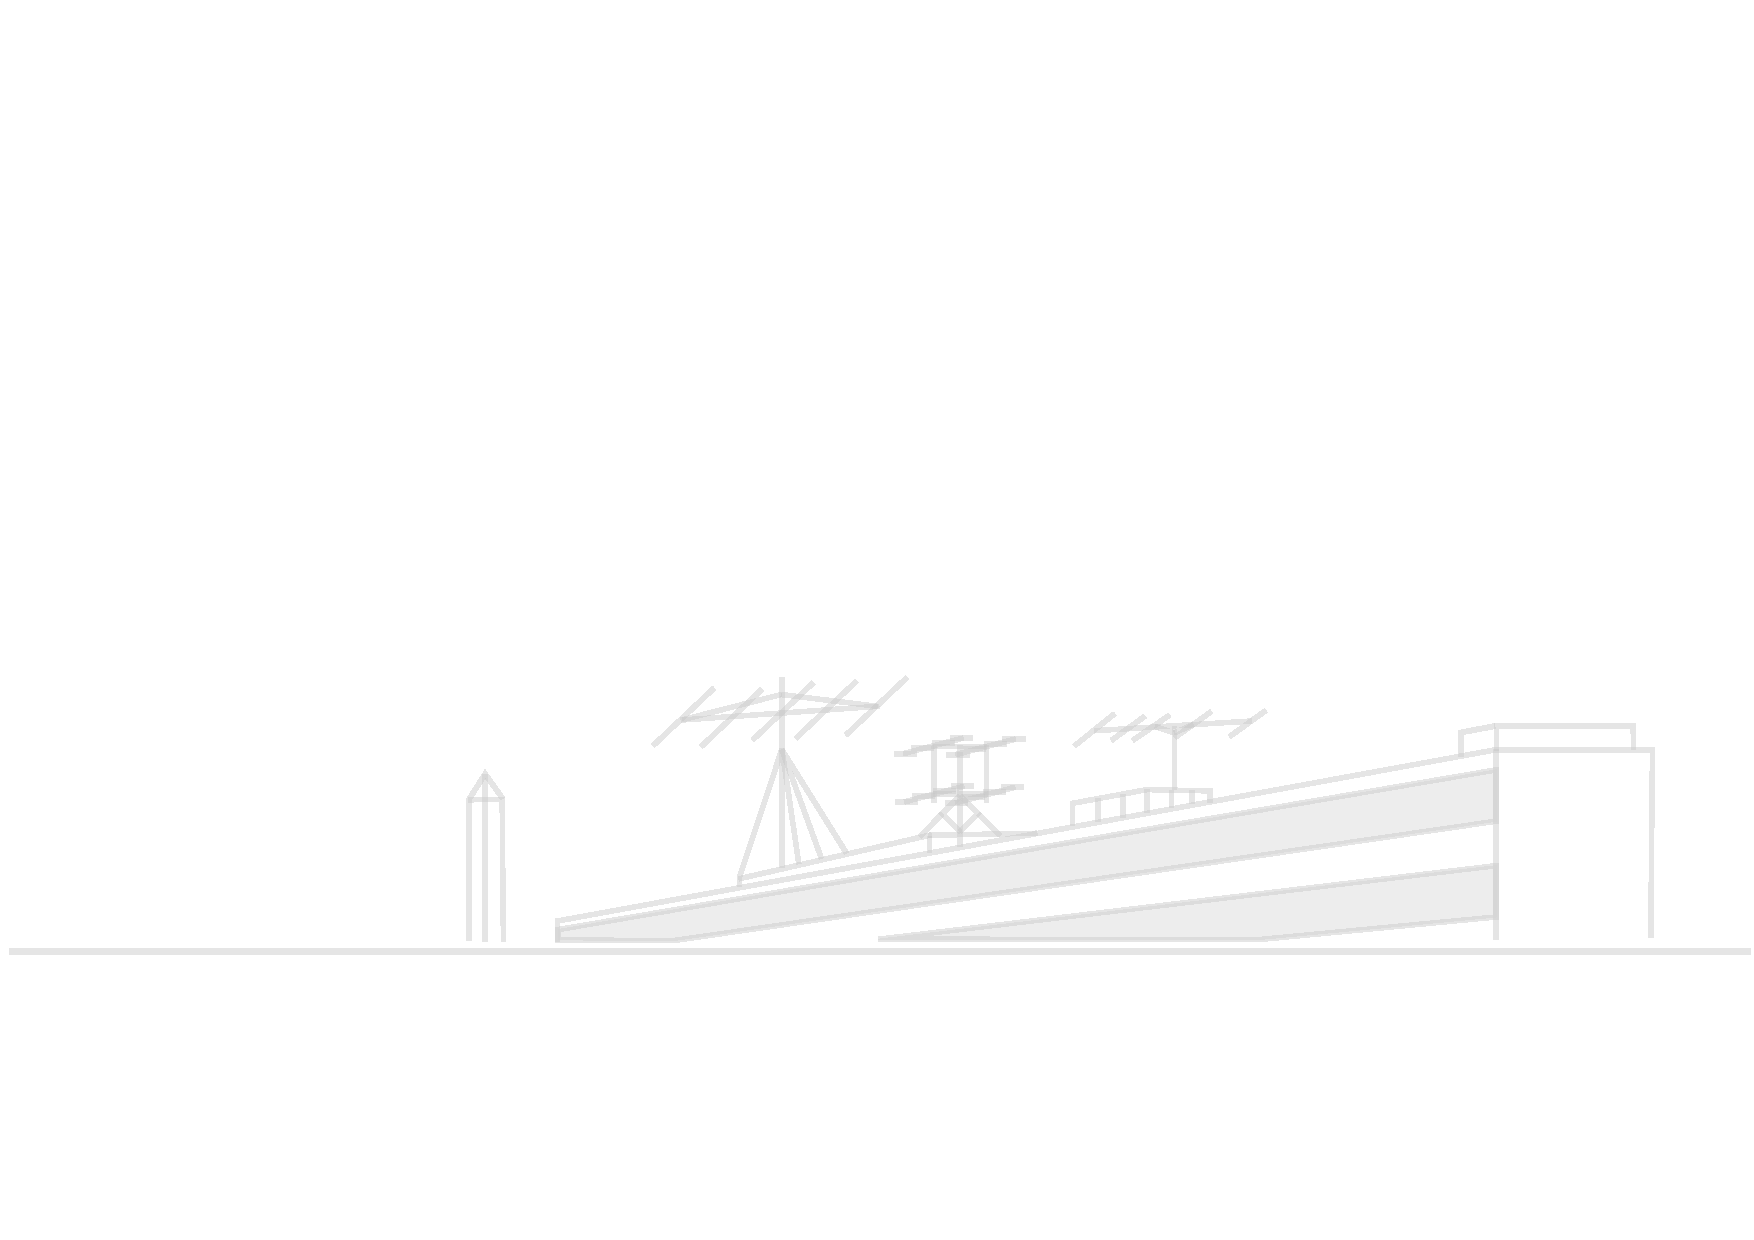
\includegraphics[width=17.8cm]{texdata/dk0tu_rooftop_background.pdf}
}

% Foliennummer einfügen
\setbeamertemplate{footline}[frame number]
%\setbeamertemplate{footline}{}

% Ändere das Zeichen vor jedem item
%\setbeamertemplate{itemize item}{\color{craneorange}$\blacktriangleright$}
%\setbeamertemplate{itemize subitem}{\color{craneorange}$\triangleright$}
%\setbeamertemplate{itemize subsubitem}{\color{craneorange}$\blacktriangleright$}

% Ändert die Blöcke 
\setbeamertemplate{blocks}[rounded][shadow=true]
% default | rounded [shadow=true|false]

%
% Eigene Kommandos
%

% Hack to get natbib and beamer working together. "The beamer user guide suggests
% that only the manual bibliography entry approach is supported"
% on some system it works out of the box, sometimes you need the hack :-(
% so check it --dl7bst
\ifdefined\newblock
    \relax
\else
    \newcommand{\newblock}{}
\fi

% \includedia command to generate png out of a dia file
% NEEDS installed dia and pdflatex option --shell-escape
\newcommand{\includedia}[1]{
    \immediate\write18{/usr/bin/dia #1.dia -e #1_diatmp.png -t png}
}

% RICHIG GROSSER FONT!
\newfont{\bigfont}{cmr10 at 144pt}
\newfont{\smallfont}{cmr10 at 8pt}

% Römische Ziffern
\makeatletter
\newcommand{\rmnum}[1]{\romannumeral #1}
\newcommand{\Rmnum}[1]{\expandafter\@slowromancap\romannumeral #1@}
\makeatother

% Schwarze Überschrift
%\setbeamercolor{frametitle}{fg=black}
%\setbeamercolor{title}{fg=black}

% Item- und Box-Farben
\definecolor{deepBlue}{HTML}{000066}
\setbeamercolor{itemize item}{fg=deepBlue}
\setbeamercolor{itemize subitem}{fg=deepBlue}
\setbeamercolor{description item}{fg=deepBlue}
\setbeamercolor{block title}{fg=deepBlue!100, bg=blue!15}
\setbeamercolor{block body}{fg=black, bg=blue!5}
\setbeamercolor{block title alerted}{fg=deepBlue, bg=red!75}
\setbeamercolor{block body alerted}{fg=black, bg=red!15}
\setbeamercolor*{block title example}{fg=blue!50, bg=blue!10}
\setbeamercolor*{block body example}{fg= blue, bg=blue!5}

%\setbeamercolor{section in head/foot}{parent=palette primary}
%\setbeamercolor{subsection in head/foot}{parent=palette secondary}
%\setbeamercolor{sidebar}{fg=darkblue,bg=yellow!90!orange}
%\setbeamercolor{title in sidebar}{fg=darkblue}
%\setbeamercolor{author in sidebar}{fg=darkblue}
%\setbeamercolor{section in sidebar}{fg=darkblue!10!black}
%\setbeamercolor{subsection in sidebar}{fg=darkblue!50!black}

% Titlepage Infos
\title{AFu-Kurs nach DJ4UF}
\author[DKØTU]{DKØTU\\ \footnotesize{Amateurfunkgruppe der TU Berlin}}
\institute[DKØTU]{\url{http://www.dk0tu.de} }

% PDF-Eigenschaften
\subject{DK0TU-Amateurfunkkurs nach DJ4UF}
\keywords{Amateurfunk Kurs HAM Radio Course CC-BY-NC-SA OpenSource TU Berlin DK0TU}

\subtitle{Technik A17: \\
           Schaltungstechnik \\[2em]}
\date{Stand 29.06.2016}
 \begin{document}

\begin{frame}
    \titlepage
    \vfill
    \begin{center}
        \ccbyncsaeu\\
        {\tiny This work is licensed under the \em{Creative Commons Attribution-NonCommercial-ShareAlike 3.0 License}.}\\[0.5ex]
         \tiny Amateurfunkgruppe der Technische Universität Berlin (AfuTUB), DKØTU
         %\includegraphics[scale=0.5]{img/DK0TU_Logo.pdf}
    \end{center}
\end{frame}


\section*{Röhren PA mit Pi-Filter}
\begin{frame}
    \frametitle{HF-Verstärker mit Röhren}
    \begin{center}
        \includegraphics[width=1\textwidth,height=.75\textheight,keepaspectratio]{a17/TG313.png}
        {\tiny \hyperlink{refs}{\cite{bna}}}\\
        Röhrenendstufe mit Pi-Filter am Ausgang (TG313)
    \end{center}
\end{frame}

\begin{frame}
  \begin{center}
    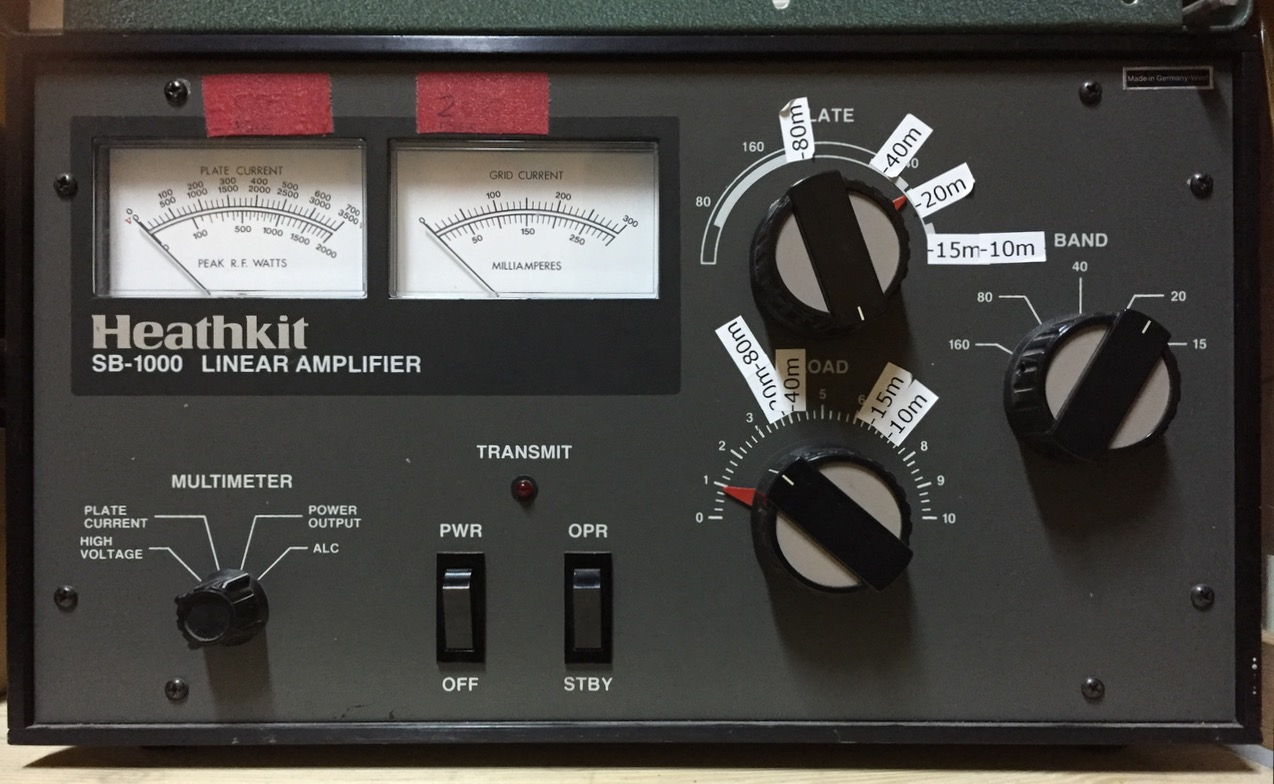
\includegraphics[width=\textwidth,height=.95\textheight,keepaspectratio]{a07/Heathkit.jpg}
    \tiny \hyperlink{refs}{\cite{dc4lw}}
  \end{center}
\end{frame}

\begin{frame}
\frametitle{Wissenswertes zu Röhren PAs mit Pi-Filtern}
\begin{center}
  \begin{itemize}
    \item haben höheren Wirkungsgrad als Transistorendstufen, da mit hohen Spannungen und geringen Strömen gearbeitet wird
    \item die meisten Verluste treten durch Ströme in den Spulen auf
    \item benötigt zur Arbeitspunkteinstellung am Gitter eine geringere Spannung als an der Katode
    \item dafür kann eine Konstantspannungsquelle oder ein Widerstand genutzt werden
    \item Pi-Filter dient der Impedanzanpassung
  \end{itemize}
\end{center}
\end{frame}

\begin{frame}
    \frametitle{Das Abstimmen einer Röhren PAs mit Pi-Filtern}

    \begin{center}
        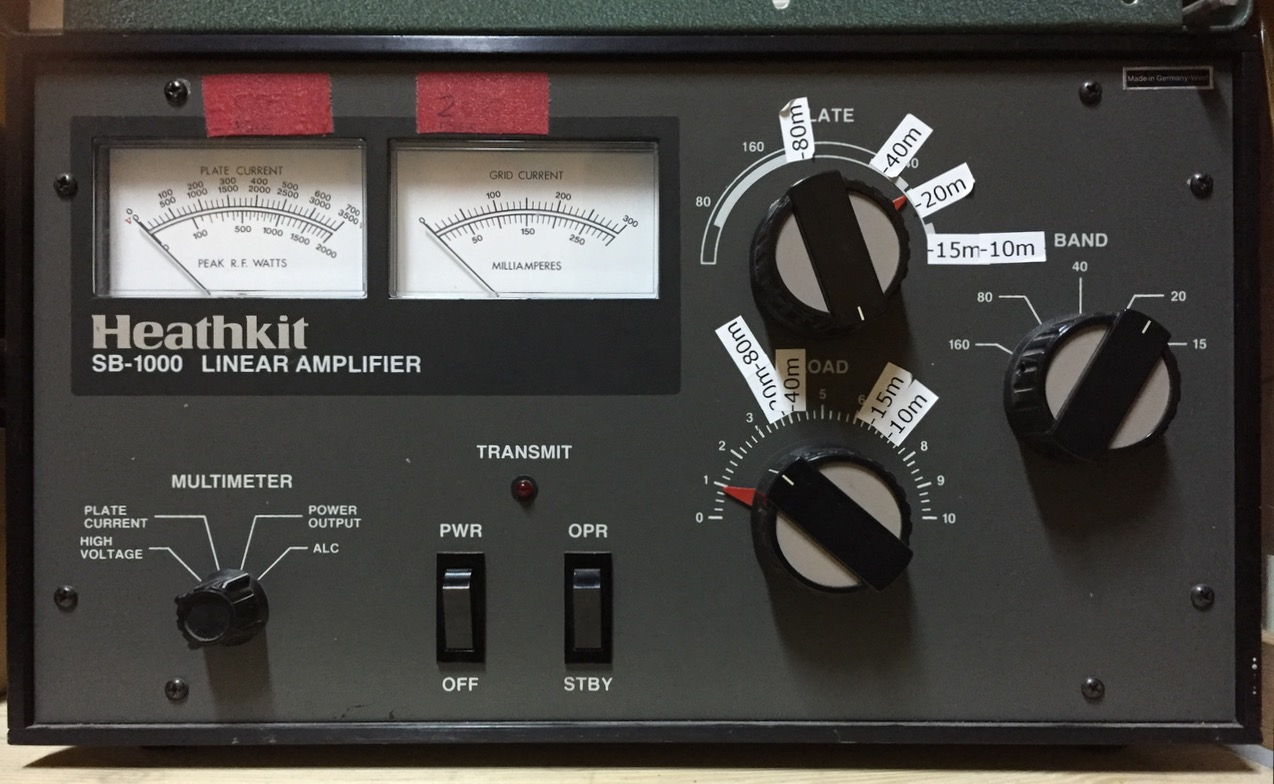
\includegraphics[width=\textwidth,height=.3\textheight,keepaspectratio]{a07/Heathkit.jpg}
        \tiny \hyperlink{refs}{\cite{dc4lw}}
    \end{center}

    \begin{itemize}
      \only<1>{
      \item $C_1$ ist für die Resonanz des Kreises verantwortlich; wird auch Abstimmkondensator, Plate oder Tune bezeichnet
      \item $C_2$ dient der Einstellung der Lastimpedanz (LOAD)
      \item Zuerst stellt man $C_1$ und $C_2$ auf max
      }
      \only<2>{
      \item $C_1$ auf Dip im Anodenstrom stellen (Resonanz); Dip heißt, der Strom ist am Minimum
      \item Nun mit $C_2$ einen etwas höheren Anodenstrom einstellen (Leistung auskoppeln)
      \item Vorgang mit $C_1$ und $C_2$ wechselseitig wiederholen bis maximale Ausgangsleistung erreicht ist
      \item Nach dem Abstimmvorgang sollte noch ein Dip von ca. 10\% verbleiben
      }
    \end{itemize}

\end{frame}

\begin{frame}
    \frametitle{Röhrenverstärker abstimmen}
    \begin{center}
        \begin{exampleblock}{TG315}
          \only<1>{Welche Bedeutung und Funktion haben $C_1$, $C_2$ und $L_1$? Wie sind die Bedienknöpfe der beiden Kondensatoren an einer Endstufe wahrscheinlich beschriftet?}
          \only<2>{An dem Drehknopf für $C_1$ steht $C_{Plate}$ oder ``Plate'', an dem für $C_2$ steht $C_{Load}$ oder ``Load''. Die drei Bauelemente $C_1$, $C_2$ und $L_1$ bilden zusammen einen so genannten Pi-Tankkreis zur Anpassung der Ausgangsimpedanz der Röhre an die Antennenimpedanz.}
        \end{exampleblock}
        \includegraphics[width=0.65\textwidth,height=.4\textheight,keepaspectratio]{a07/TG313.png}
        {\tiny TG313--TG318 \hyperlink{refs}{\cite{bna}}}
      \end{center}
\end{frame}

\begin{frame}
    \frametitle{Röhrenverstärker abstimmen}
    \begin{center}
      \begin{exampleblock}{TG316}
        \only<1>{Wie wird die folgende Endstufe richtig auf die Sendefrequenz abgestimmt?}
        \only<2>{Zum Abstimmen $C_1$ und $C_2$ auf maximale Kapazität stellen. $C_1$ auf Dip im Anodenstrom (Resonanz) stellen, dann mit $C_2$ einen etwas höheren Anodenstrom einstellen (Leistung auskoppeln). Vorgang mit $C_1$ und $C_2$ wechselweise mehrmals wiederholen bis die maximale Ausgangsleistung erreicht ist. Nach dem Abstimmvorgang sollte ein Dip von etwa $10\%$ verbleiben.}
      \end{exampleblock}
      \includegraphics[width=0.6\textwidth,height=.4\textheight,keepaspectratio]{a07/TG313.png}
      {\tiny TG313--TG318 \hyperlink{refs}{\cite{bna}}}
    \end{center}
\end{frame}

\begin{frame}
  \begin{tabular}{l||p{.8\textwidth}}\hline
    \textbf{TG310} & \textbf{LC-Schaltungen unmittelbar vor und hinter einem HF-Leistungsverstärker dienen}\\ \hline\hline
    A & zur Verringerung der rücklaufenden Leistung bei Fehlanpassung. \\ \hline
    B & zur optimalen Einstellung des Arbeitspunktes nach Betrag und Phase. \\ \hline
    C \only<2>\checkmark & zur optimalen Anpassung der Ein- und Ausgangsimpedanzen. \\ \hline
    D & zur Erhöhung des HF-Wirkungsgrades der Verstärkerstufe. \\ \hline
  \end{tabular}
\end{frame}

\section*{2m-FM Endstufe}
\begin{frame}
  \frametitle{2m-FM Endstufe}
    \begin{center}
        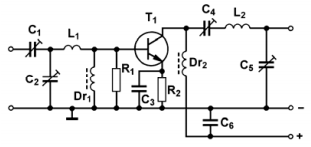
\includegraphics[width=0.7\textwidth,height=.7\textheight,keepaspectratio]{a17/TG311.png}
        {\tiny TG311--TG312 \hyperlink{refs}{\cite{bna}}}\\
        $2m$-FM Endstufe
    \end{center}
\end{frame}
\begin{frame}
\frametitle{2m-FM Endstufe abgleichen}
\begin{itemize}
  \item zum Abgleich des Verstärkers wird eine $50 \Omega$ Dummy-Load für UKW angeschlossen
  \item dann wird die Eingangsleistung erhöht, bis der Strom etwas ansteigt
  \item nun abwechselnd die Ausgangskondensatoren verstellen bis die Leistung etwa konstant bleibt
  \item danach wird der Vorgang mit den Eingangskondensatoren wiederholt
  \item dann wird die Eingangsleistung erhöht bis die Schaltung einen Strom von etwa $2,7 A$ aufnimmt (= Nennstrom der Schaltung)
  \item anschließend wird der Abgleich mit dem nun eingestellten Strom wiederholt
  \item um Eigenschwingungen zu vermindern kann man die Eingangsimpedanz des Transistors mit einem Widerstand dämpfen
  \item oder den Emitteranschluss mit einer Ferritperle versehen
\end{itemize}
\end{frame}

\begin{frame}
\frametitle{2m-FM Endstufe in der Praxis}
\begin{itemize}
  \item Schaltung sollte in ein Metallgehäuse montiert werden
  \item am Besten noch mit Trennwand hinter dem Transistor
  \item Verstärker arbeitet im C-Betrieb
  \item kann nur CW und FM -- \textbf{kein SSB}
\end{itemize}
\end{frame}

\begin{frame}
  \begin{tabular}{l||p{.8\textwidth}}\hline
    \textbf{TG312} & \textbf{Welche der nachfolgenden Aussagen trifft \underline{nicht} für die Schaltung zu?}

        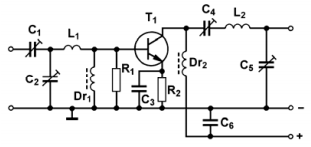
\includegraphics[width=.5\textwidth,height=.5\textheight,keepaspectratio]{a17/TG311.png} \\ \hline\hline
    A & HF-Eingang und HF-Ausgang sind gleichspannungsfrei. \\ \hline
    B & $C_4$, $C_5$ und $L_2$ passen den Transistorausgang an die niederohmigere Ausgangsimpedanz an. \\ \hline
    C & $C_1$, $C_2$ und $L_1$ passen die hochohmigere Eingangsimpedanz an den Transistoreingang an. \\ \hline
    D \only<2>\checkmark & $R_1$ dient zur Arbeitspunkteinstellung des Transistors $T_1$. \\ \hline
  \end{tabular}
\end{frame}


\section*{Linearverstärker}
\begin{frame}
  \frametitle{Linearverstärker}
    \begin{center}
        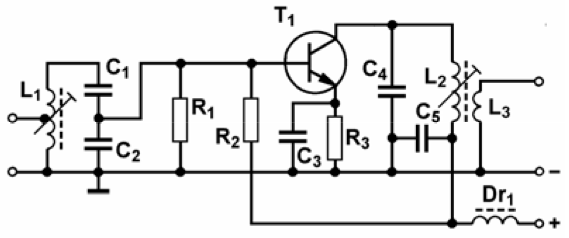
\includegraphics[width=.8\textwidth,height=.8\textheight,keepaspectratio]{a17/TG222.png}
        {\tiny TG222--TG225 \cite{bna}}
    \end{center}
\end{frame}

\begin{frame}
\frametitle{Linearverstärker}
\begin{itemize}
  \item für den SSB-Betrieb geeignet
  \item HF-Verstärker sollen möglichst verzerrungsfrei (linear) verstärken
  \item einen solchen Verstärker kann man mit zwei Transistoren im Gegentakt-B-Betrieb aufbauen
  \item oder mit einem Transistor im AB-Betrieb
  \item bei kleinen Signalen arbeitet der Transistor dann im A-Betrieb und bei größeren im B-Betrieb
  \item $R_1$ und $R_2$ bestimmen den Arbeitspunkt des Transistors
  \item der Schwingkreis $L_1$--$C_1$--$C_2$ schafft eine doppelte Resonanztransformation
  \item das Verhältnis von $C_1$ zu $C_2$ bestimmt die Anpassung an die Basis des Transistors
  \item die Mittelanzapfung an $L_1$ erzeugt den üblichen $50 \Omega$ Eingangswiderstand
  \item der Ausgang wird normal transformiert über $L_2$ zu $L_3$
\end{itemize}
\end{frame}

\begin{frame}
  \begin{tabular}{l||p{.8\textwidth}}\hline
    \textbf{TG222} & \textbf{Bei dieser Schaltung handelt es sich um einen}

      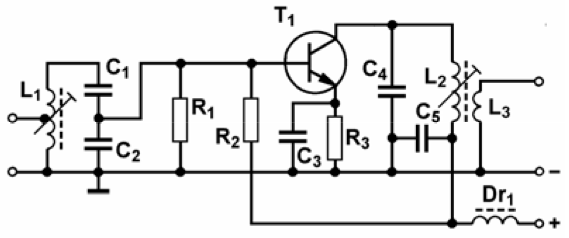
\includegraphics[width=.5\textwidth,height=.5\textheight,keepaspectratio]{a17/TG222.png} \\ \hline\hline
    A & Oszillator. \\ \hline
    B & Mischer. \\ \hline
    C & NF-Verstärker. \\ \hline
    D \only<2>\checkmark & HF-Verstärker. \\ \hline
  \end{tabular}
\end{frame}

\begin{frame}
  \begin{tabular}{l||p{.8\textwidth}}\hline
    \textbf{TG223} & \textbf{Welchem Zweck dient $C_5$ in der folgenden Schaltung?}

      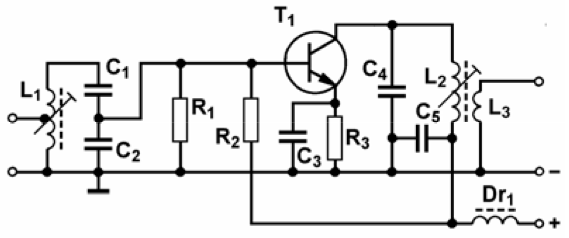
\includegraphics[width=.5\textwidth,height=.5\textheight,keepaspectratio]{a17/TG222.png} \\ \hline\hline
    A \only<2>\checkmark & Zur HF-Entkopplung. \\ \hline
    B & Zur Abstimmung. \\ \hline
    C & Zur Wechselstromkopplung. \\ \hline
    D & Zur Kopplung mit der nächstfolgenden Stufe. \\ \hline
  \end{tabular}
\end{frame}

\begin{frame}
  \begin{tabular}{l||p{.8\textwidth}}\hline
    \textbf{TG224} & \textbf{Welchem Zweck dient die Anzapfung an $L_1$ in der folgenden Schaltung?}

      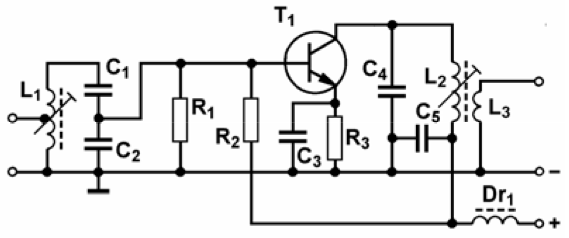
\includegraphics[width=.5\textwidth,height=.5\textheight,keepaspectratio]{a17/TG222.png} \\ \hline\hline
    A \only<2>\checkmark & Sie dient zur Anpassung der Eingangsimpedanz der Stufe. \\ \hline
    B & Sie schützt die Verstärkerstufe vor wilden Schwingungen. \\ \hline
    C & Sie bewirkt die notwendige Entkopplung für den Schwingungseinsatz der Oszillatorstufe. \\ \hline
    D & Sie dient zur Erhöhung des HF-Wirkungsgrades der Verstärkerstufe. \\ \hline
  \end{tabular}
\end{frame}

\begin{frame}
  \begin{tabular}{l||p{.8\textwidth}}\hline
    \textbf{TG225} & \textbf{Welchem Zweck dient $C_2$ in der folgenden Schaltung?}

      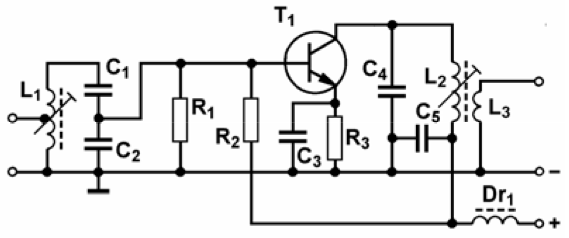
\includegraphics[width=.5\textwidth,height=.5\textheight,keepaspectratio]{a17/TG222.png} \\ \hline\hline
    A \only<2>\checkmark & Zur Festlegung der HF-Kopplung. \\ \hline
    B & Zur Verhinderung der Schwingneigung. \\ \hline
    C & Zur Gleichstromentkopplung. \\ \hline
    D & Zur Unterdrückung von Oberwellen. \\ \hline
  \end{tabular}
\end{frame}

\section*{Detektor-Empfänger}
\begin{frame}
  \frametitle{Der Detektorempfänger}
    \begin{center}
        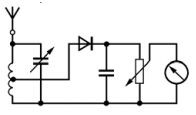
\includegraphics[width=.7\textwidth,height=.7\textheight,keepaspectratio]{a17/TJ601.png}
        {\tiny TJ601 \cite{bna}}
    \end{center}
\end{frame}


\section*{Oszillatoren}
\begin{frame}
\frametitle{Aufbau von Oszillatoren}
\begin{itemize}
  \item Spulen und Kondensatoren sind temperaturabhängig
  \item Spulen dehnen sich aus, dadurch steigt ihr Querschnitt und die Induktivität
  \item deshalb nutzt man dafür Kondensatoren mit negativen Temperaturkoeffizienten, wie z.B. Styroflexkondensatoren
  \item dies alles beeinflusst die Frequenz
  \item also, Oszillatoren weg von Wärmequellen!
  \item extra stabilisierte Spannungsversorgung verhindert ein Verzerren der Frequenz durch den Transistor
  \item und immer gut schirmen
\end{itemize}
\end{frame}

\begin{frame}
  \begin{tabular}{l||p{.8\textwidth}}\hline
    \textbf{TD611} & \textbf{``Chirp'' ist eine Form der Frequenzinstabilität. Es wird hervorgerufen durch} \\ \hline\hline
    A & Phasensprung der Oszillatorfrequenz durch zu steile Flanken des Tastsignals. \\ \hline
    B & Frequenzänderungen des Oszillators, weil die Tastung auf der falschen Stufe erfolgt. \\ \hline
    C \only<2>\checkmark & Frequenzänderungen des Oszillators z.B.\,durch zu schwach ausgelegte Stromversorgung. \\ \hline
    D & Kontaktprellungen am Tastrelais. \\ \hline
  \end{tabular}
\end{frame}

\begin{frame}
  \begin{tabular}{l||p{.8\textwidth}}\hline
    \textbf{TG209} & \textbf{Beim Bau eines VFO sollte die Spule} \\ \hline\hline
    A & so fest wie möglich um einen Kern aus rostfreiem Stahl gewickelt werden. \\ \hline
    B & locker um einen Keramikkern gewickelt werden. \\ \hline
    C & neben einem Ventilator angebracht werden, um sie zu kühlen. \\ \hline
    D \only<2>\checkmark & in einer Position angeordnet werden, die möglichst geringen Temperaturschwankungen unterworfen ist. \\ \hline
  \end{tabular}
\end{frame}

\begin{frame}
  \begin{tabular}{l||p{.8\textwidth}}\hline
    \textbf{TK106} & \textbf{Alle Geräte, die HF-Ströme übertragen, sollten} \\ \hline\hline
    A \only<2>\checkmark & möglichst gut geschirmt sein. \\ \hline
    B & nicht geerdet sein. \\ \hline
    C & über das Stromversorgungsnetz geerdet sein. \\ \hline
    D & durch Kunststoffabdeckungen geschützt sein. \\ \hline
  \end{tabular}
\end{frame}

\begin{frame}
  \begin{tabular}{l||p{.8\textwidth}}\hline
    \textbf{TF404} & \textbf{Die Spule, die Bestandteil des frequenzbestimmenden Elementes eines VFO ist, sollte} \\ \hline\hline
    A \only<2>\checkmark & eine solide mechanische Konstruktion aufweisen. \\ \hline
    B & aus Widerstandsdraht bestehen. \\ \hline
    C & freitragend sein. \\ \hline
    D & um einen Stahlkern gewickelt sein. \\ \hline
  \end{tabular}
\end{frame}

\section*{Dummy-Load}

\begin{frame}
\frametitle{Die Dummy-Load}
\begin{columns}
  \column[c]{.4\textwidth}
  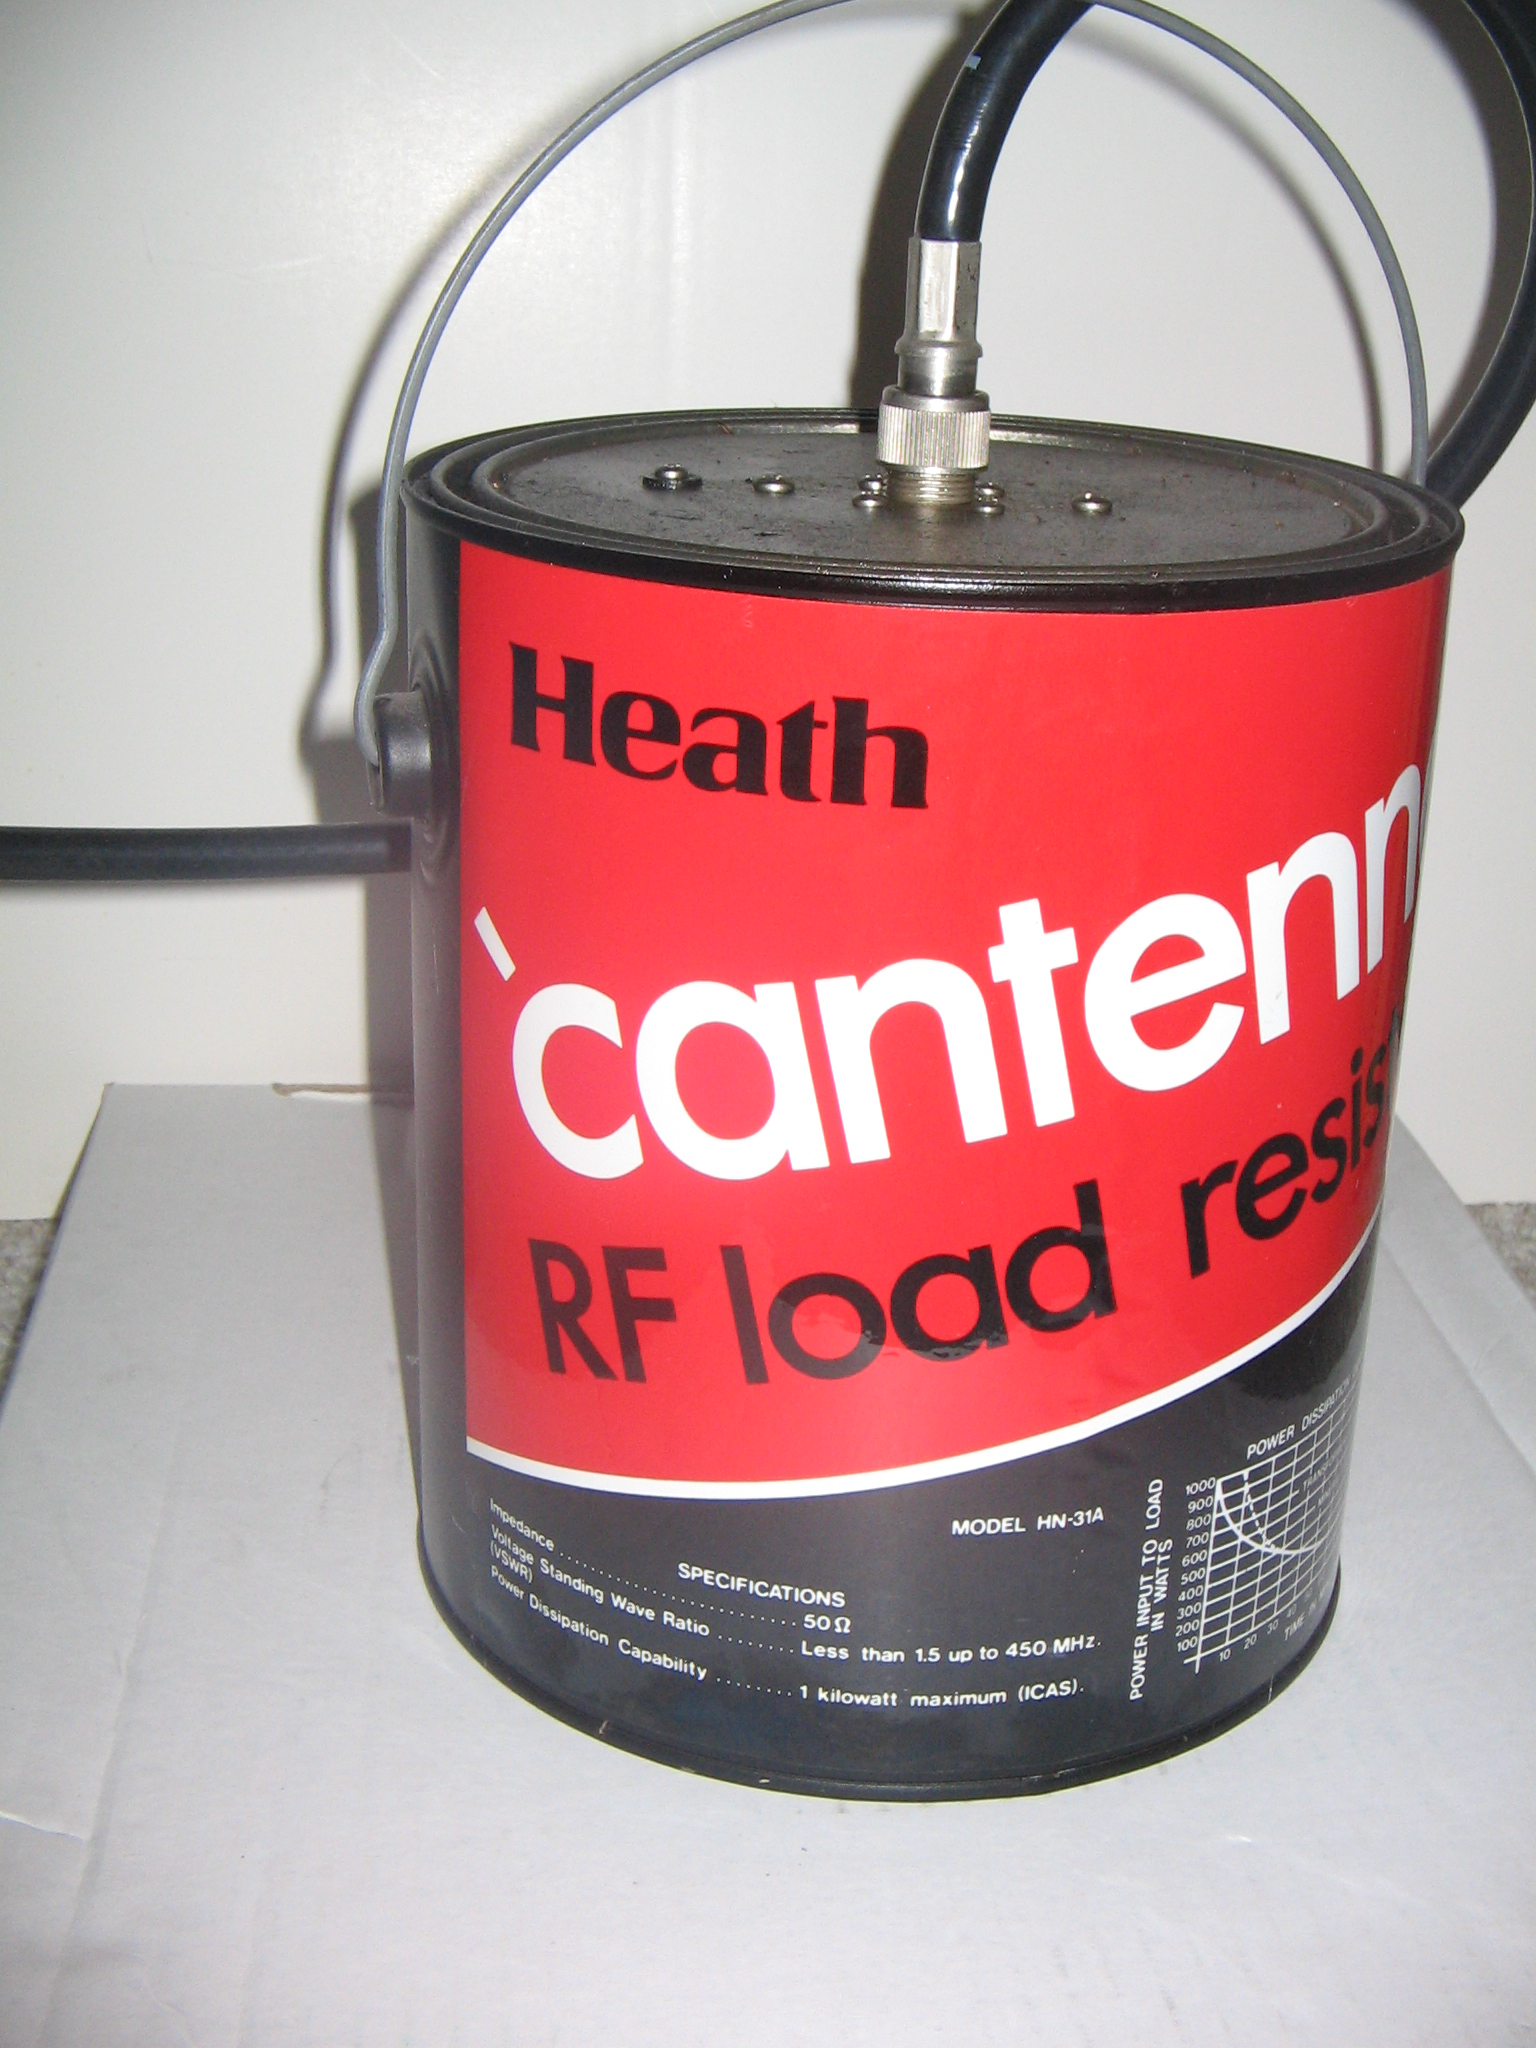
\includegraphics[width=\textwidth,height=.8\textheight,keepaspectratio]{a17/Cantenna.JPG}\\
  \centering Cantenna \cite{wm}
  \column[c]{.55\textwidth}
  \begin{itemize}
    \item im Prinzip ist die Dummy-Load ein Widerstand für hohe Frequenzen und Leistungen
    \item dabei soll sie wenig kapazitive und -- noch wichtiger -- wenig induktive Anteile haben
    \item gut eignen sich Schichtwiderstände
    \item Aufbau als Widerstandskaskade mit $50\Omega$
  \end{itemize}
\end{columns}
\end{frame}

\begin{frame}
  \begin{tabular}{l||p{.8\textwidth}}\hline
    \textbf{TJ708} & \textbf{Für den Bau einer Dummy Load wurden Schichtwiderstände von 150\,Ohm\,/\,1\,Watt verwendet. Jeweils vier Widerstände wurden in Serie geschaltet und durch Parallelschaltung dieser Serienschaltungen wurden zirka 50\,Ohm erreicht. Wie viele Widerstände wurden insgesamt benötigt und welche Dauerleistung verträgt die Dummy Load?}

    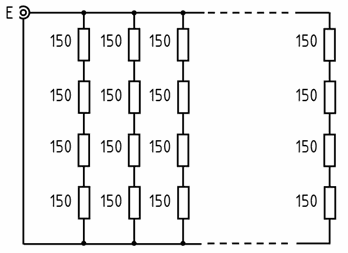
\includegraphics[width=.8\textwidth,height=.43\textheight,keepaspectratio]{a17/tj708.png}\\ \hline\hline
    A & gesamt 48 Widerstände, 12 Watt \\ \hline
    B \only<2>\checkmark & gesamt 48 Widerstände, 48 Watt \\ \hline
    C & gesamt 12 Widerstände, 48 Watt \\ \hline
    D & gesamt 16 Widerstände, 16 Watt \\ \hline
  \end{tabular}
\end{frame}

\section*{Netzteil und Stabilisierung}
\begin{frame}
  \frametitle{Netzteil und Stabilisierung}
    \begin{center}
        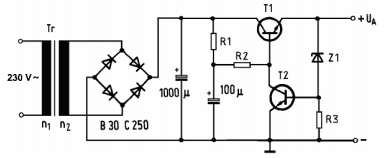
\includegraphics[width=1\textwidth,height=.43\textheight,keepaspectratio]{a17/TD306.png}
        {\tiny Netzteil aus TD306 \hyperlink{refs}{\cite{bna}}}
    \end{center}
    Wie funzt das?
\begin{itemize}
  \item Die Ausgangsspannung wird als Vergleich zur Transistorsteuerung genommen
  \item Fixe Ausgangspannung $\equiv$ Z-Diodenspannung + $0,6V$ $U_{BE}$ für $T_2$
  \item $U_A$ sinkt (bei höherer Belastung) $\rightarrow$ $I_{B,T2}$ sinkt (und leitet weniger) $\rightarrow$ $U_{R_1,R_2}$ sinkt (durch verminderten Kollektorstrom an T2) $\rightarrow$ $U_{B,T1}$ steigt $\rightarrow$ $T1$ leitet besser $\rightarrow$ $U_A$ steigt
\end{itemize}
\end{frame}

\subsection*{Fest"-pannungs"-regler}
\begin{frame}
  \frametitle{Festspannungsregler}
  \begin{columns}
    \column[c]{.5\textwidth}
      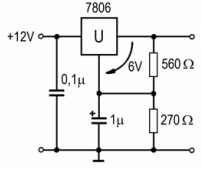
\includegraphics[width=1\textwidth,height=.8\textheight,keepaspectratio]{a17/TD319.png}\\
      {\tiny Festpannungsregler aus TD319 \hyperlink{refs}{\cite{bna}}}
    \column{.45\textwidth}
    \begin{itemize}
      \item viel freundlicher im Umgang als z.B. die Z-Diodenschaltung
      \item benötigen nur noch Kondensatoren drum herum
      \item brauchen etwa $15\%$ mehr Eingangsspannung als sie stabilisieren sollen
      \item sollte der Regler mal zu wenig Strom liefern, kann er mit einem Transistor erweitert werden
      \item Bauteil: 78xx-Serie (und 79xx für negative Spannungen)
    \end{itemize}
  \end{columns}
\end{frame}

\begin{frame}
  \begin{tabular}{l||p{.8\textwidth}}\hline
    \textbf{TD319} & \textbf{Welche Ausgangsspannung entsteht mit folgender Spannungsregler-Schaltung?}

    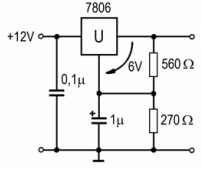
\includegraphics[width=.5\textwidth,height=.45\textheight,keepaspectratio]{a17/TD319.png} \\ \hline\hline
    A & 6\,V \\ \hline
    B \only<2>\checkmark & 8,9\,V \\ \hline
    C & 18\,V \\ \hline
    D & 14,9\,V \\ \hline
  \end{tabular}
  \pause
  Der Trick: am Mittelanschluss wird ein höheres Potenzial zum Vergleich angelegt. $6V$ von 7806 fallen auch über die $560\Omega$ ab. Strom von $10,7mA$ entsteht. Fließt durch $270\Omega$, wo $2,89V$ entstehen, die zu den $6V$ dazu addiert werden.
\end{frame}

\begin{frame}
  \begin{tabular}{l||p{.8\textwidth}}\hline
    \textbf{TTD312} & \textbf{Die Ausgangsspannung zwischen A und B in der Schaltung beträgt ungefähr}

    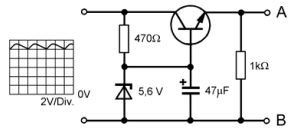
\includegraphics[width=.6\textwidth,height=.6\textheight,keepaspectratio]{a17/TD312.png} \\ \hline\hline
    A & 5,6 Volt. \\ \hline
    B & 11,2 Volt. \\ \hline
    C & 6,2 Volt. \\ \hline
    D \only<2>\checkmark & 5 Volt. \\ \hline
  \end{tabular}
  \pause
  Z-Diode stabilisiert auf $5,6V$. Transistor braucht $0,6V$.
\end{frame}


\subsection*{Schaltnetzteil}
\begin{frame}
    \begin{center}
        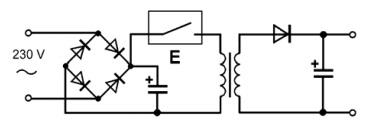
\includegraphics[width=.7\textwidth,height=.5\textheight,keepaspectratio]{a17/TD317.png}
        {\tiny Schaltnetzteil aus TD317 \hyperlink{refs}{\cite{bna}}}
    \end{center}
    \begin{itemize}
      \item will man den Trafo in einem Netzteil verkleinern, brauch man höhere Spannungen
      \item Lösung des Problems: man richtet die Wechselspannung gleich, zerhackstückelt diese dann per elektronischen Schalter, transformiert sie dann und richtet sie wieder gleich
      \item Schaltfrequenzen gehen bis in den MHz-Bereich
      \item erzeugt dafür aber Oberwellen, die auf KW stören können
    \end{itemize}
\end{frame}

\begin{frame}
  \begin{tabular}{l||p{.8\textwidth}}\hline
    \textbf{TD317} & \textbf{Welche Funktion hat der Block E bei einem Schaltnetzteil?}

    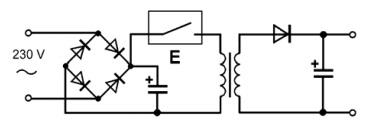
\includegraphics[width=.6\textwidth,height=.5\textheight,keepaspectratio]{a17/TD317.png}\\ \hline\hline
    A & Er wandelt die Wechselspannung in Gleichspannung um. \\ \hline
    B & Er soll bei Überspannungen den Transformator schützen. \\ \hline
    C \only<2>\checkmark & Es ist ein elektronischer Schalter zur Pulsweitensteuerung. \\ \hline
    D & Er dient als Puls-Gleichrichter in dieser Schaltung. \\ \hline
  \end{tabular}
\end{frame}

\section*{Mechanik \& Sicherheit}
\begin{frame}
\frametitle{Was für die Bastler}
\begin{itemize}
  \item \textbf{Immer an die Abschirmung denken!}
  \item am besten Metallgehäuse nutzten
  \item braucht das Gerät Netzspannung, muss das gesamte Gehäuse geerdet werden
  \item bei HF-Verstärkern in der Versorgung auch noch die HF rausfiltern
\end{itemize}
\end{frame}

\begin{frame}
  \begin{tabular}{l||p{.8\textwidth}}\hline
    \textbf{TD316} & \textbf{Bei der Verbindung der Stromversorgung mit HF-Leistungsverstärkern ist} \\ \hline\hline
    A & eine Schutzdiode vorzusehen. \\ \hline
    B & eine separate Erdung vorzusehen. \\ \hline
    C & eine zusätzliche Schmelzsicherung vorzusehen. \\ \hline
    D \only<2>\checkmark & eine genügende HF-Filterung vorzusehen. \\ \hline
  \end{tabular}
\end{frame}

\begin{frame}
  \begin{tabular}{l||p{.8\textwidth}}\hline
    \textbf{TF408} & \textbf{Um Einrichtungen mit einem Klappdeckel aus Metall möglichst gut abzuschirmen, empfiehlt es sich, das Scharnier} \\ \hline\hline
    A \only<2>\checkmark & mit einem guten Erdband zu überbrücken. \\ \hline
    B & das Halteband mit einer Ferritperle zu versehen. \\ \hline
    C & mit einem Polystyrol-Kondensator abzublocken. \\ \hline
    D & mit einem Kunststoffhalter zu versehen. \\ \hline
  \end{tabular}
\end{frame}

\begin{frame}
  \begin{tabular}{l||p{.8\textwidth}}\hline
    \textbf{TF419} & \textbf{Die Stabilität des lokalen Oszillators einer Sende"~/""Empfangsanalage ist teilweise von} \\ \hline\hline
    A \only<2>\checkmark & einer robusten mechanischen Konstruktion abhängig. \\ \hline
    B & der Verwendung von Tantalkondensatoren für die frequenzbestimmenden Teile abhängig. \\ \hline
    C & der Verwendung von Widerstandsdraht für die Spule abhängig. \\ \hline
    D & einer niederohmigen Gleichstromversorgung des VFO abhängig. \\ \hline
  \end{tabular}
\end{frame}

\begin{frame}
  \begin{tabular}{l||p{.8\textwidth}}\hline
    \textbf{TG514} & \textbf{Um die Gefahr von Eigenschwingungen in HF-Schaltungen zu verringern,} \\ \hline\hline
    A & sollten die Abschirmungen der einzelnen Stufen nicht miteinander verbunden werden. \\ \hline
    B \only<2>\checkmark & sollte jede Stufe gut abgeschirmt sein. \\ \hline
    C & sollten die Betriebsspannungen den einzelnen Stufen mit koaxialen oder verdrillten Leitungen zugeführt werden. \\ \hline
    D & sollte jede Stufe eine eigene stabilisierte Stromversorgung haben. \\ \hline
  \end{tabular}
\end{frame}

\begin{frame}
  \begin{tabular}{l||p{.8\textwidth}}\hline
    \textbf{TF427} & \textbf{Um unerwünschte Abstrahlungen auf ein Minimum zu beschränken, sollte eine Mischstufe} \\ \hline\hline
    A \only<2>\checkmark & gut abgeschirmt sein. \\ \hline
    B & niederfrequent entkoppelt werden. \\ \hline
    C & nicht geerdet werden. \\ \hline
    D & mit gut gesiebter Gleichspannung gespeist werden. \\ \hline
  \end{tabular}
\end{frame}

\begin{frame}
  \begin{tabular}{l||p{.8\textwidth}}\hline
    \textbf{TG306} & \textbf{Die Ausgangsanpassschaltung und das Filter eines HF-Verstärkers im C-Betrieb sollten} \\ \hline\hline
    A \only<2>\checkmark & in einem auf Masse liegenden Metallkasten untergebracht werden. \\ \hline
    B & hinter dem Verstärker aufgestellt werden, um die Kühlung zu verbessern. \\ \hline
    C & vor dem Verstärker eingebaut werden. \\ \hline
    D & direkt an der Antenne befestigt werden. \\ \hline
  \end{tabular}
\end{frame}

\begin{frame}
  \begin{tabular}{l||p{.8\textwidth}}\hline
    \textbf{TF429} & \textbf{Um unerwünschte Abstrahlungen eines Oszillators zu vermeiden, sollte} \\ \hline\hline
    A & er niederohmig HF-entkoppelt sein. \\ \hline
    B & er nicht abgeschirmt werden. \\ \hline
    C \only<2>\checkmark & er in einem Metallkasten untergebracht werden. \\ \hline
    D & die Speisespannung gesiebt sein. \\ \hline
  \end{tabular}
\end{frame}

\begin{frame}
  \begin{tabular}{l||p{.8\textwidth}}\hline
    \textbf{TG218} & \textbf{Stufen, in denen Harmonische erzeugt werden, sollten} \\ \hline\hline
    A & sehr gute Mantelwellenfilter enthalten. \\ \hline
    B \only<2>\checkmark & sehr sorgfältig abgeschirmt sein. \\ \hline
    C & in Polystyrol eingegossen werden. \\ \hline
    D & eine besonders gesiebte Spannungsstabilisierung erhalten. \\ \hline
  \end{tabular}
\end{frame}

\begin{frame}
  \begin{tabular}{l||p{.8\textwidth}}\hline
    \textbf{TL101} & \textbf{In Bezug auf EMV sollten Vervielfacherstufen} \\ \hline\hline
    A \only<2>\checkmark & gut abgeschirmt sein. \\ \hline
    B & eine besonders abgeschirmte Spannungsversorgung erhalten. \\ \hline
    C & in Kunststoff eingehüllt sein. \\ \hline
    D & nur kapazitive Auskopplungen enthalten. \\ \hline
  \end{tabular}
\end{frame}

\begin{frame}
  \begin{tabular}{l||p{.8\textwidth}}\hline
    \textbf{TL102} & \textbf{Um eine Amateurfunkstelle in Bezug auf EMV zu optimieren} \\ \hline\hline
    A \only<2>\checkmark & sollten alle Einrichtungen mit einer guten HF-Erdung versehen werden. \\ \hline
    B & sollte der Sender mit der Wasserleitung im Haus verbunden werden. \\ \hline
    C & sollten alle schlechten Erdverbindungen entfernt werden. \\ \hline
    D & sollten die Wasserleitungsanschlüsse aus Polyäthylen zur Isolation vorgesehen werden. \\ \hline
  \end{tabular}
\end{frame}

\renewcommand{\refname}{Referenzen}

\hypertarget{refs}{}
\textcolor{white}{} \\ %\vspace{} geht nicht
\Large Referenzen/Links
\footnotesize

\begin{thebibliography}{}
  \bibitem{darc}  DARC Online-Lehrgang Lektion A17:
    \url{http://www.darc.de/referate/ajw/ausbildung/darc-online-lehrgang/technik-klasse-a/technik-a17/}
  \bibitem{wm} 	Wikimedia:\\
    \href{https://commons.wikimedia.org/wiki/File:Cantenna.JPG?uselang=de}{Cantenna, von No machine-readable author provided. Gerry Ashton assumed (based on copyright claims). [GFDL (http://www.gnu.org/copyleft/fdl.html), CC-BY-SA-3.0 (http://creativecommons.org/licenses/by-sa/3.0/) oder CC BY-SA 2.5-2.0-1.0 (http://creativecommons.org/licenses/by-sa/2.5-2.0-1.0)], via Wikimedia Commons}
  \bibitem{bna}   Fragenkatalog Bundesnetzagentur Technik Klasse A:
    \url{https://www.bundesnetzagentur.de/SharedDocs/Downloads/DE/Sachgebiete/Telekommunikation/Unternehmen_Institutionen/Frequenzen/Amateurfunk/Fragenkatalog/TechnikFragenkatalogKlasseAf252rId9014pdf.pdf?__blob=publicationFile&v=3}
  \bibitem{fi}    Freie Inhalte (DK0TU):
    \url{http://www.dk0tu.de/Projekte/Freie_Inhalte/}
  \bibitem{dc4lw} eigene Aufnahme DC4LW
\end{thebibliography}

% Hier könnte noch eine Kontaktfolie stehen

\end{document}

